% This is appa.tex
%
% This file is for appendices.  If you don't have any appendices, delete
% the percent sign from the beginning of the next line.
%\endinput

\clearpage
\appendix
\section{Appendix: Figures, Tables and Algorithms}

\begin{figure}[h!]
    \centering
    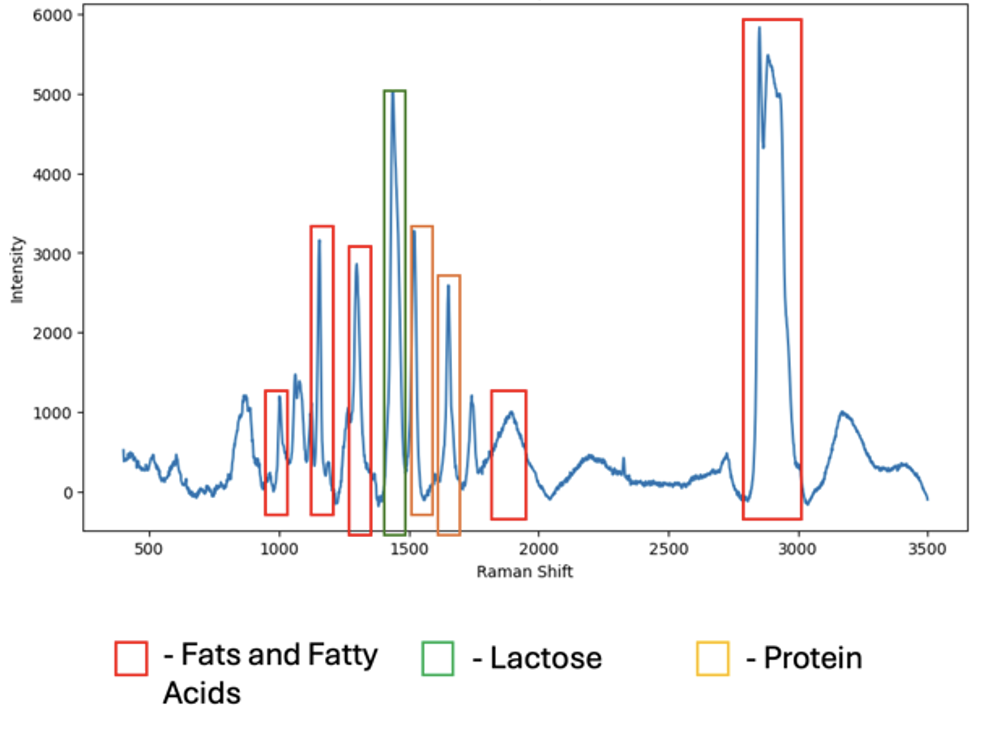
\includegraphics[width=0.5\linewidth]{Figures/Screenshot 2025-07-16 at 2.26.41 PM.png}
    \caption{Characterization of Raman Peaks for the Control Sample: The three primary constituents are proteins, fats and sugars.}
    \label{fig:ram}
\end{figure}

\begin{table}[h!]
\centering
\begin{tabular}{|l|c|l|}
\hline
\textbf{Functional Groups} & \textbf{Raman Band (cm\textsuperscript{-1})} & \textbf{Component} \\
\hline
Aromatic C--C & 1016 & Fat \\
CH\textsubscript{2} twist, Ester & 1279, 1315 & Fat \\
CH\textsubscript{2} bending & 1416, 1759 & Fat, Lactose \\
Amide I & 1566 & Proteins \\
Amide II & 1670 & Proteins \\
CH stretch & 2865, 2902 & Fatty Acids \\
\hline
\end{tabular}
\caption*{Table 1A: Raman spectral bands of various functional groups in milk components}
\label{tab:raman_bands}
\end{table}


\begin{figure}[h!]
    \centering
    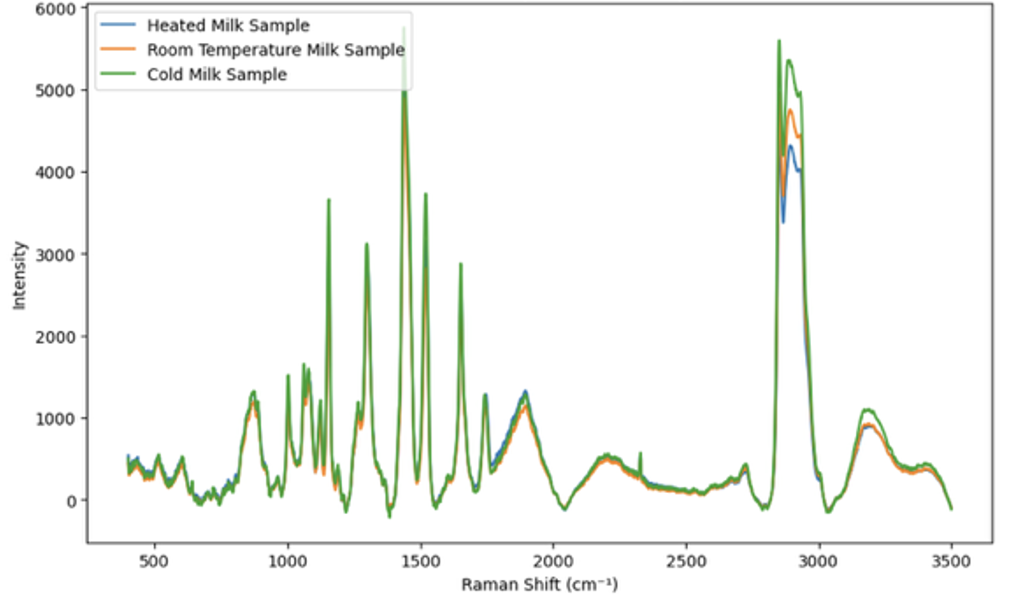
\includegraphics[width=0.5\linewidth]{Figures/Screenshot 2025-07-16 at 2.27.09 PM.png}
    \caption{Variation in Raman Spectra of Control Sample with Temperature. Fatty Acid content varies directly with temperature.}
    \label{fig:temp}
\end{figure}

\begin{figure}[h!]
    \centering
    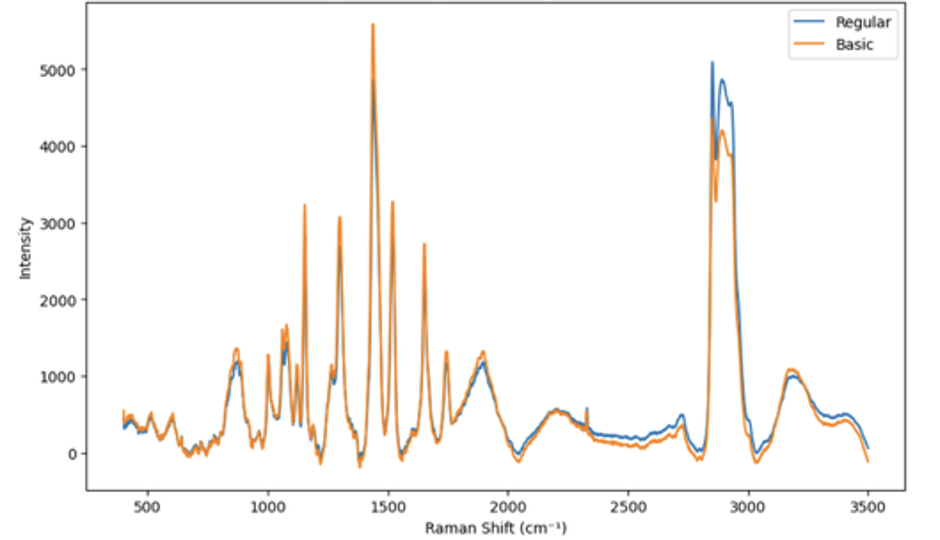
\includegraphics[width=0.5\linewidth]{Figures/Screenshot 2025-07-16 at 2.27.24 PM.png}
    \caption{Variation in Raman Spectra of Control Sample with pH indicating variation in peak between 2800 and 3000 $cm^{-1}$}
    \label{fig:confusion}
\end{figure}

\begin{figure}
    \centering
    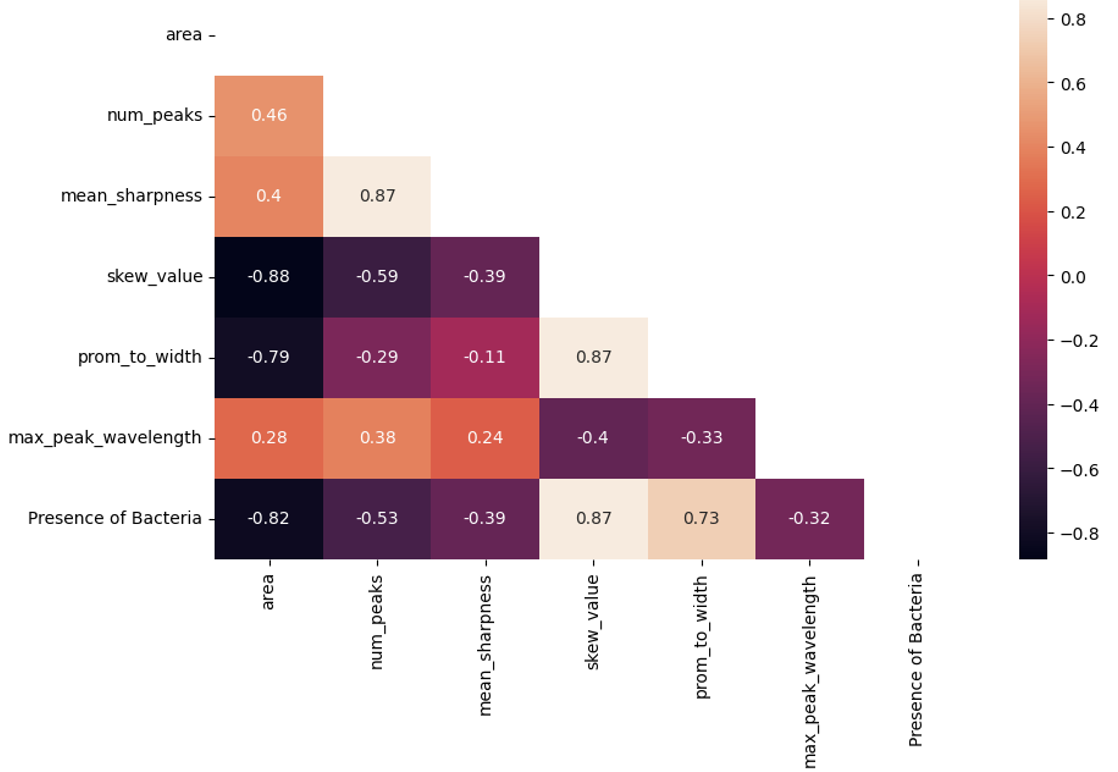
\includegraphics[width=0.5\linewidth]{Figures/Screenshot 2025-07-16 at 2.27.59 PM.png}
    \caption{Correlation Analysis of Feature Extracted Variables. Area and Skewness show maximum correlation with the target variable.}
    \label{fig:corr}
\end{figure}

\begin{figure}
    \centering
    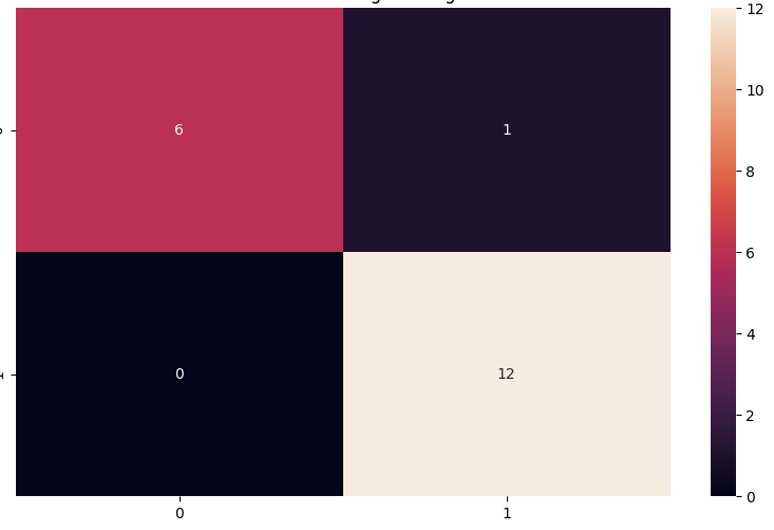
\includegraphics[width=0.5\linewidth]{Figures/Screenshot 2025-07-16 at 2.28.32 PM.png}
    \caption{Confusion Matrix for Logistic Regression, Support Vector Machines and Naive Bayes Classifier}
    \label{fig:cm}
\end{figure}

\begin{figure}
    \centering
    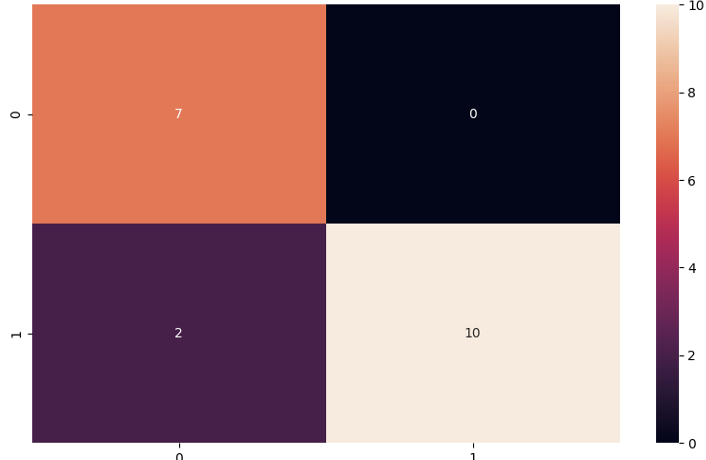
\includegraphics[width=0.5\linewidth]{Figures/Screenshot 2025-07-16 at 2.28.53 PM.png}
    \caption{Confusion Matrix for Gaussian Process Classifiers}
    \label{fig:cm2}
\end{figure}

\begin{table}[h!]
\centering
\begin{tabular}{|l|p{10cm}|}
\hline
\textbf{Milk Type} & \textbf{Conditions} \\
\hline
Amul Toned & Heated to 60°C, Cooled to 4°C, 7 pH, Bacteria \\
Amul Fresh Cream & Heated to 60°C, Cooled to 4°C, 7 pH \\
Heritage Toned & Heated to 60°C, Cooled to 4°C, 7 pH, Bacteria \\
Heritage Fresh Cream & Heated to 60°C, Cooled to 4°C, 7 pH, Bacteria, Bacteria Low Concentration \\
Heritage Special & Heated to 60°C, 7 pH, 6.2 pH, Bacteria \\
Nandini Toned & Heated to 60°C, Cooled to 4°C, 7 pH, Bacteria \\
Nandini Full Cream & Heated to 60°C, Cooled to 4°C, 7 pH, Bacteria \\
Nestle Toned & Heated to 60°C, Cooled to 4°C, 7 pH \\
Akshaykalpa & Bacteria \\
\hline
\end{tabular}
\caption*{Table 2A: Conditions applied to different types of milk samples}
\label{tab:milk_conditions}
\end{table}

\begin{algorithm}
\caption{Raman Spectrum Feature Extraction}
\begin{algorithmic}[1]
\State \textbf{Input:} Preprocessed Raman spectra matrix $S$ of shape $(n_{\text{samples}}, n_{\text{points}})$
\State \textbf{Output:} Feature matrix $F$ of shape $(n_{\text{samples}}, n_{\text{features}})$
\For{each spectrum $s$ in $S$}
    \State Compute area under the curve: $ \text{area} \gets \texttt{integrate}(s)$
    \State Identify all peaks: $ \text{peaks} \gets \texttt{find\_peaks}(s, \text{height} = \text{threshold})$
    \State Initialize $ \text{sharpness\_list} \gets [\;]$
    \For{each peak in peaks}
        \State Compute sharpness: $ \text{sharpness} \gets \frac{\text{height}}{\text{width\_at\_half\_max}}$
        \State Append sharpness to list: $ \text{sharpness\_list.append(sharpness)}$
    \EndFor
    \State Compute mean peak sharpness: $ \text{mean\_sharpness} \gets \texttt{mean}( \text{sharpness\_list})$
    \State Compute max peak sharpness: $ \text{max\_sharpness} \gets \texttt{max}( \text{sharpness\_list})$
    \State Count number of peaks: $ \text{num\_peaks} \gets \texttt{length}(\text{peaks})$
    \State Find position of max intensity peak: $ \text{max\_peak\_pos} \gets \texttt{argmax}(s)$
    \State Compute skewness: $ \text{skewness} \gets \texttt{skew}(s)$
    \State Store features in matrix $F$:
    \Statex \hspace{\algorithmicindent}$F[i] \gets [\text{area}, \text{mean\_sharpness}, \text{max\_sharpness},$
    \Statex \hspace{\algorithmicindent} \phantom{$F[i] \gets [$}$\text{num\_peaks}, \text{max\_peak\_pos}, \text{skewness}]$
\EndFor
\State \Return $F$
\end{algorithmic}
\label{alg:feature_extraction}
\end{algorithm}

\begin{table}[h]
\centering
\begin{tabular}{|l|l|}
\hline
\textbf{Feature} & \textbf{p-value} \\
\hline
Area & $1.92639 \times 10^{-24}$ \\
Peaks & $5.2382 \times 10^{-8}$ \\
Mean sharpness & $1.0916 \times 10^{-4}$ \\
Skewness & $5.93292 \times 10^{-30}$ \\
Sharpness of most prominent peak & $7.36415 \times 10^{-17}$ \\
Wavelength corresponding to max intensity & $1.449561 \times 10^{-3}$ \\
\hline
\end{tabular}
\caption*{Table 3A: Two-tailed t-test p-values for key Raman spectral features.}
\label{tab:ttest_pvalues}
\end{table}


\begin{table}[htbp]
\centering
\begin{tabular}{|l|c|}
\hline
\textbf{Model} & \textbf{Accuracy (\%)} \\
\hline
Logistic Regression & 95 \\
Naive Bayes & 95 \\
SVM & 95 \\
Random Forest & 100 \\
GPC & 89 \\
KNN & 100 \\
\hline
\end{tabular}
\caption*{Table 4A: Accuracy of different ML Models suing Feature Extracted Data.}
\label{tab:feacc}
\end{table}

\begin{figure}[htbp]
  \centering
  \begin{subfigure}[b]{0.45\textwidth}
    \centering
    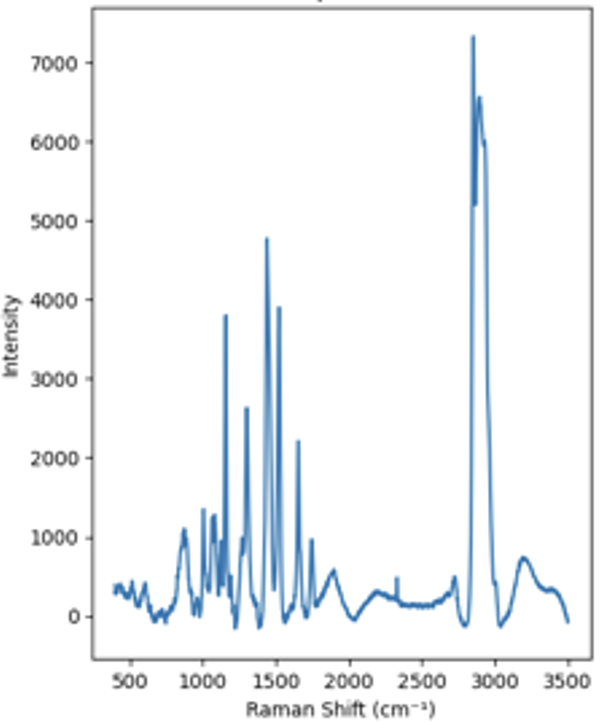
\includegraphics[scale=0.6]{Figures/HORIBA.png}
    \caption{Spectra from Lab 1}
    \label{fig: horiba}
  \end{subfigure}
  \hfill
  \begin{subfigure}[b]{0.45\textwidth}
    \centering
    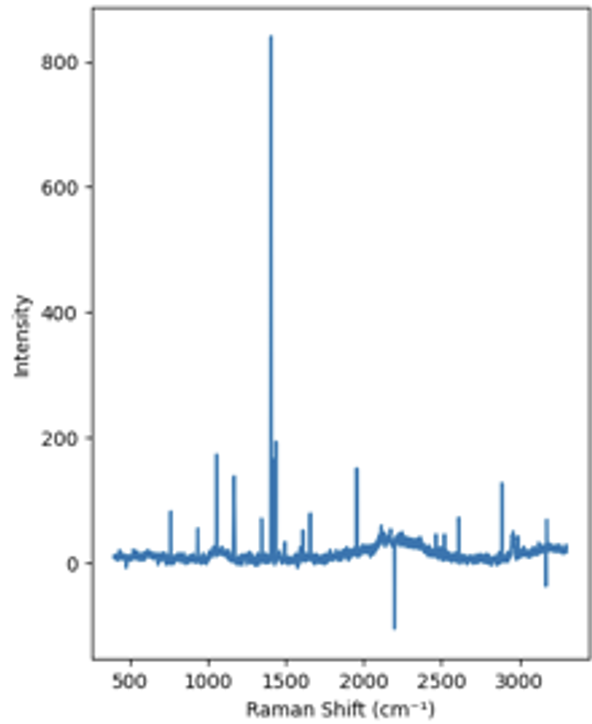
\includegraphics[scale=0.6]{Figures/Sampath.png}
    \caption{Spectra from Lab 2}
    \label{fig:sampath}
  \end{subfigure}
  \caption{Confounding Variable in Data Collection. The Spectrum from Lab 2 shows greater spectral noise than spectra from Lab 1.}
  \label{fig:combined3}
\end{figure}

\begin{figure}
    \centering
    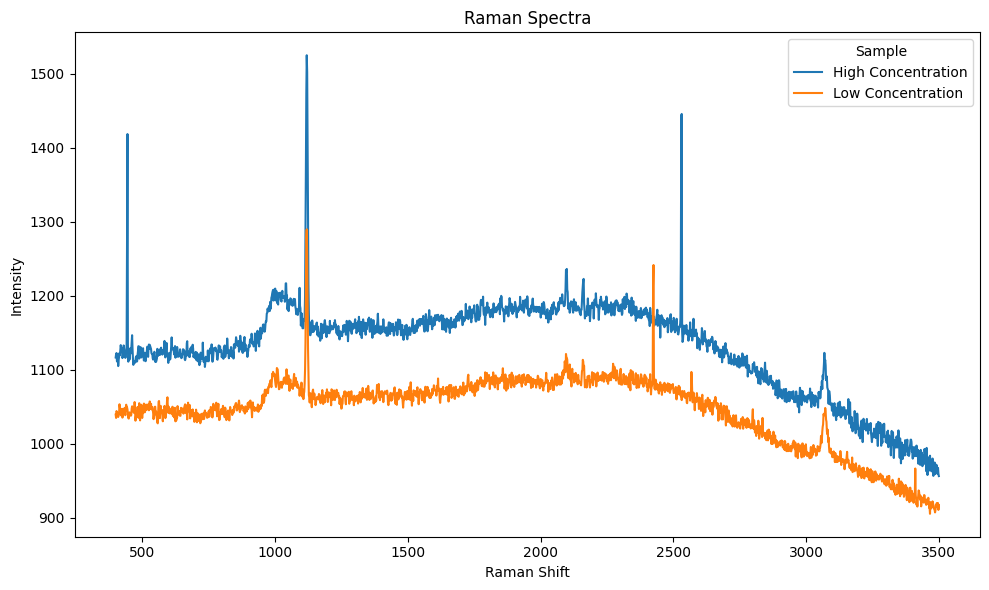
\includegraphics[scale = 0.5]{Figures/concentration variation.png}
    \caption{Variation in Spectra with Concentration. The primary difference is in the intensities.}
    \label{fig:conc}
\end{figure}